\chapter{Princípios de Usabilidade}

Os princípios de design e os princípios de usabilidade constituem os fundamentos teóricos e práticos essenciais para o desenvolvimento de interfaces de usuário eficazes e experiências digitais significativas. Em um cenário onde as expectativas dos usuários evoluem continuamente e as tecnologias digitais se tornam cada vez mais complexas, a compreensão e aplicação adequada destes princípios torna-se crucial para o sucesso de produtos digitais.


\section{Princípios de usabilidade}

A usabilidade refere-se à medição de quão facilmente um usuário pode alcançar seus objetivos ao usar um serviço \cite{digital_gov_usability}. Isso geralmente é medido através de metodologias de pesquisa estabelecidas sob o termo "teste de usabilidade", que inclui taxas de sucesso e satisfação do cliente. A usabilidade é uma parte do guarda-chuva mais amplo da experiência do usuário (UX). Enquanto UX abrange o design da experiência geral de um produto, a usabilidade foca na mecânica de garantir que os produtos funcionem da melhor forma possível para o usuário.
\begin{comment}
Doze princípios de usabilidade padrão da indústria são usados para avaliar formalmente a usabilidade de sistemas, aplicações e interfaces \cite{stanford_usability}. Estes princípios são informados por várias diretrizes de usabilidade da indústria, incluindo princípios consistentes que nos permitem alinhar melhor aos padrões aprimorados para experiência do usuário.

	Este capítulo introduz os fundamentos do design para usabilidade e UX, focando na aplicação de ciência, arte e artesanato ao seu design fundamentado \cite{researchgate_usability_ux}. Ele revisa os principais métodos de avaliação de usabilidade, focando em testes de usabilidade. O conceito de UX lança uma rede ampla sobre todas as experiências do usuário.
\end{comment}

Em 2024, o tema "Designing for a Better World" com foco em usabilidade, sustentabilidade e inclusividade pôde ser visto em vários contextos \cite{world_usability_day}. Esta abordagem contemporânea reflete a crescente consciência sobre a responsabilidade social do design e a necessidade de criar soluções que não apenas funcionem bem, mas também contribuam positivamente para a sociedade.

Os designers são encorajados a se manterem atualizados com estes princípios para atender às expectativas evolutivas dos usuários e entregar soluções digitais impactantes \cite{medium_ui_principles_2025}. A evolução contínua da tecnologia e das expectativas dos usuários requer uma abordagem dinâmica à aplicação de princípios de design e usabilidade.

\section{Princípios de design}

Os princípios de design referem-se aos fundamentos teóricos e diretrizes práticas que orientam a criação de interfaces visuais e funcionais eficazes. Em 2024, o design de interface de usuário (UI) enfatiza princípios como design centrado no usuário, acessibilidade e simplicidade para aprimorar experiências digitais \cite{slideshare_ui_principles_2024}. As principais tendências também incluem design responsivo, micro-interações e a integração de personalização e design de movimento para criar interfaces envolventes e sustentáveis.

O design de interface de usuário bem-sucedido torna-se mais fácil quando você compreende os 14 princípios fundamentais de design de UI, começando pelo design para o usuário \cite{uxpin_ui_principles}. Estes princípios fornecem uma estrutura conceitual que permite aos designers tomarem decisões informadas e criarem soluções que atendam tanto às necessidades funcionais quanto às expectativas estéticas dos usuários.
\begin{comment}
	Como designer de UX, você deve priorizar a usabilidade sobre a estética. Incorpore testes de usabilidade no processo de design para identificar (e corrigir) problemas de usabilidade, garantindo uma experiência do usuário amigável e eficiente em geral \cite{ux_design_institute}. Os sete princípios de UX design devem ser mantidos em mente para alcançar resultados efetivos.
\end{comment}

Muitos designers e educadores de Interface de Usuário (UI) discutem princípios a serem seguidos ao projetar os aspectos funcionais de uma UI \cite{tandfonline_ui_principles}. No entanto, muitos princípios de UI foram propostos, espalhados na literatura científica, criando a necessidade de uma abordagem unificada para a compreensão e aplicação destes conceitos.

\section{Avaliação Heurística}
A avaliação heurística constitui-se como um método de inspeção de usabilidade amplamente reconhecido no campo da Interação Humano-Computador (IHC), desenvolvido originalmente por Jakob Nielsen e Rolf Molich em 1990 \cite{nielsen1990heuristic}. Este método fundamenta-se na análise sistemática de interfaces através da aplicação de princípios heurísticos estabelecidos, permitindo a identificação de problemas de usabilidade sem a necessidade direta de envolvimento de usuários finais durante o processo de avaliação \cite{nielsen1994usability}.

As dez heurísticas de usabilidade de Nielsen representam o conjunto mais amplamente aplicado na literatura de IHC, abrangendo aspectos fundamentais como visibilidade do status do sistema, correspondência entre sistema e mundo real, controle e liberdade do usuário, consistência e padrões, prevenção de erros, reconhecimento ao invés de memorização, flexibilidade e eficiência de uso, design estético e minimalista, auxílio aos usuários no reconhecimento, diagnóstico e recuperação de erros, e disponibilização de ajuda e documentação \cite{nielsen1995ten}.

A aplicação da avaliação heurística envolve tipicamente a participação de três a cinco especialistas em usabilidade, que examinam independentemente a interface e identificam violações dos princípios heurísticos \cite{nielsen1994finding}. Este método oferece vantagens significativas em termos de custo-benefício, rapidez de aplicação e capacidade de identificação de problemas críticos de usabilidade durante as fases iniciais do desenvolvimento de sistemas interativos \cite{zhang2003comparison}.

\section{Avaliação de Acessibilidade Digital}
A avaliação de acessibilidade digital representa um domínio especializado da IHC que se concentra na garantia de que interfaces e sistemas computacionais sejam utilizáveis por pessoas com diferentes tipos de deficiência e limitações funcionais \cite{petrie2007accessibility}. Esta área fundamenta-se nos princípios de design universal e inclusivo, visando eliminar barreiras que possam impedir ou dificultar o acesso de usuários com deficiências visuais, auditivas, motoras ou cognitivas aos recursos tecnológicos.

As Diretrizes de Acessibilidade para Conteúdo Web (WCAG) 2.1, desenvolvidas pelo World Wide Web Consortium (W3C), estabelecem o padrão internacional mais reconhecido para avaliação de acessibilidade digital \cite{w3c2018wcag}. Estas diretrizes fundamentam-se em quatro princípios básicos: perceptibilidade (informações e componentes da interface devem ser apresentados de forma que os usuários possam percebê-los), operabilidade (componentes da interface e navegação devem ser operáveis), compreensibilidade (informações e operações da interface devem ser compreensíveis), e robustez (conteúdo deve ser suficientemente robusto para ser interpretado por uma ampla variedade de tecnologias assistivas).

A avaliação de acessibilidade emprega métodos combinados que incluem inspeção automatizada através de ferramentas especializadas, avaliação manual por especialistas em acessibilidade, e testes com usuários reais utilizando tecnologias assistivas como leitores de tela, navegação por teclado e dispositivos de entrada alternativos \cite{abascal2019inclusive}. A integração de critérios de acessibilidade no processo de desenvolvimento de aplicações móveis torna-se particularmente relevante considerando que dispositivos móveis representam frequentemente a principal forma de acesso à tecnologia digital para pessoas com deficiência \cite{trewin2013mobile}.

\section{Integração de Usabilidade e Acessibilidade no Desenvolvimento de Aplicações}
A convergência entre avaliação de usabilidade e acessibilidade no contexto de desenvolvimento de aplicações móveis representa uma abordagem holística que reconhece a interconexão entre facilidade de uso e inclusividade digital \cite{power2012equal}. Esta integração é particularmente crítica no desenvolvimento de aplicações de segurança e emergência, onde a usabilidade deficiente pode comprometer a eficácia da ferramenta em situações críticas, e barreiras de acessibilidade podem excluir usuários em situações de vulnerabilidade.

Metodologias contemporâneas de avaliação combinam princípios heurísticos tradicionais com critérios específicos de acessibilidade, resultando em frameworks integrados que abordam simultaneamente eficiência, eficácia, satisfação do usuário e inclusividade \cite{yesilada2015evaluating}. A aplicação destes métodos no contexto de aplicações de segurança pessoal requer consideração especial para cenários de uso sob estresse, limitações temporais críticas, e diversidade de perfis de usuários que podem incluir pessoas com diferentes capacidades funcionais e níveis de letramento digital. E a avaliação de acessibilidae que visa garantir o uso por qualquer usuário.

\section{Usabilidade SheSafe}
\begin{comment}
	Você tem que deixar claro que essas telas fazem parte do projeto inicial e que procurou colocar elementos nas telas de modo a atender os princípios de usabilidade, mas não precisa ficar dizendo qual é qual.
\end{comment}
Foram realizadas três avaliações principais para o aplicativo SheSafe: A avaliação de rapída e rasteira, encontrada no anexo B, visa fazer uma tomada rápida de opinião e oferecer aos interessados indicações gerais sobre a qualidade da experiência do usuário. A avaliação de usabilidade, encontrada no anexo A, que tem o objetivo de verificar o que acontece com o usuário. E o teste de acessibilidade, encontrado no anexo C, que tem como objetivo a verificação do uso do aplicativo por qualquer usuário.

A seguir é possível ver as telas que fazem parte do wireframe do projeto inicial da interface. Nas telas foram inseridos elementos que atendem aos princípios de usabilidae e os reforçam.
\subsection{Tela 1 - Home}
\begin{figure}[h]
  \begin{center}
  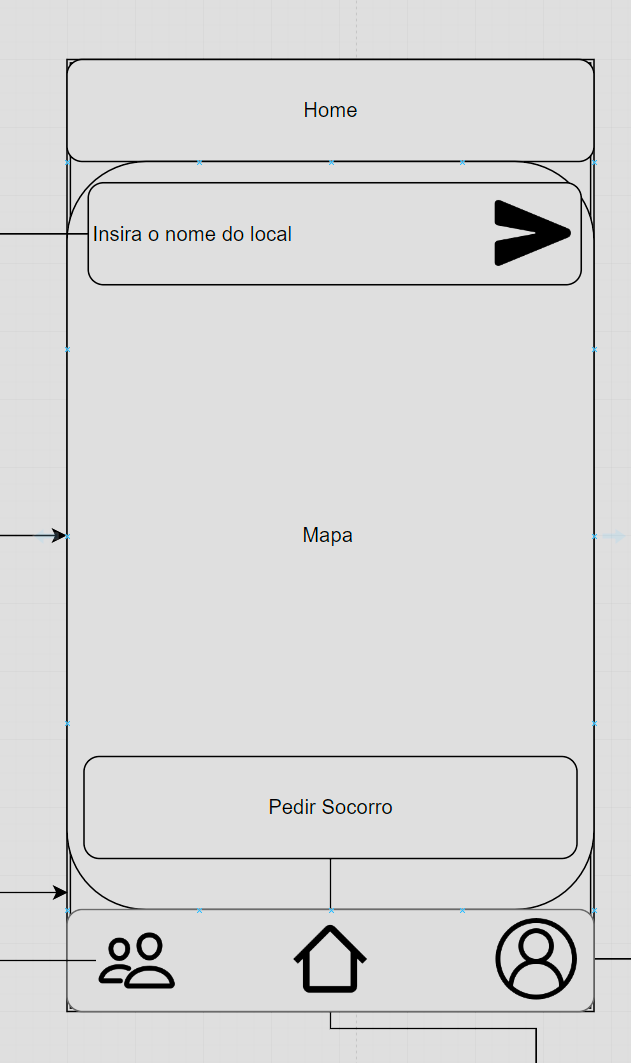
\includegraphics[width=0.2\linewidth]{images/wire-tela-home.png}\\
  \end{center}
  \caption[Wireframe Tela Home]{Wireframe Tela Home}
  \label{fig:wireframe-tela-home}
  \legend{Fonte: Próprio Autor}
\end{figure}
\pagebreak
\begin{comment}
	\begin{alineas}
		\item Tipo de interface e interação
		
		Na tela home será utilizada o tipo de tela de interface gráfica onde o usuário irá visualizar sua localização atual no mapa e um campo de busca e um botão de pedido de socorro. A forma de interação será através de toque nos botões tanto da bottom bar quanto do pedir socorro. E através de formulário no campo para inserir o nome do local a ser buscado.
		\item Metáforas
		
		A BottomBar contém ícones os quais remetem as funcionalidades do aplicativo. O ícone com dois bonecos remete a uma lista de contatos. O ícone da casa remete a tela principal de qualquer aplicativo. Já o ícone circular com boneco dentro remete ao perfil em qualquer aplicação. A própria BottomBar já remete a ideia de que é possível navegar entre essas três telas sem que tenha que sair deste menu em si. 
		\item Aprendizibilidade
		
		Previsibilidade – Ao clicar em qualquer um dos ícones da bottom bar o usuário será navegado para a tela correspondente ao ícone.
		
		Capacidade de sintetização – O usuário receberá um alert em formato de notificação Toast ao clicar em enviar pedido de socorro e confirmar (caso a confirmação de envio esteja ativada) que deseja enviar.
		
		Familiaridade – Não se aplica.
		
		Consistência – A bottom bar será apresentada sempre no fim das três telas principais (contatos, home e perfil). E os seus ícones estarão sempre na mesma ordem de posição.
		
		Generalização – Não se aplica.
		\item Flexibilidade
		
		Iniciativa de diálogo – É possível cancelar o pedido de socorro ao clicar em cancelar (caso a confirmação de envio esteja ativada).
		
		Multitarefa – Não se aplica.
		
		Migração de atividades – Não se aplica.
		
		Substitutividade – Não se aplica.
		
		Personalização – Não se aplica.
		\item Robustez
		
		Observabilidade – O mapa indicará a localização atual do usuário na tela home.
		
		Recuperabilidade – O sistema irá emitir um alert em formato de Toast indicando quando houver falha no envio de um pedido de socorro e pedirá para que o usuário refaça a solicitação.
		
		Capacidade de resposta – Ao enviar ou confirmar um pedido de socorro o sistema irá emitir um alerta em formato de Toast indicando que o pedido foi enviado.
		
		Conformidade de realização de atividades – O usuário irá receber na tela um aviso em caso de perda de conexão e pedirá que o usuário se reconecte antes de continuar as operações. 
	\end{alineas}
\end{comment}
Na tela home será utilizada a interface gráfica onde será possível o usuário visualizar um mapa com sua localização atual. Haverá um campo de busca e um botão para acionamento do pedido de socorro. Toda a interação será realizada através de toque nos botões da bottom bar, no botão de pedido de socorro e no formulário de busca.

A bottom bar conterá três ícones que represetam as funcionalidade principais do aplicativo. O ícone com dois bonecos remete a lsita de contatos. O ícone da casa remete a tela principal nos aplicativos que utilizam tal ícone. Já o ícone circular com boneco remete ao perfil nos aplicativos em que é utilizado. A própri abottom bar já consiste na idea de uma interface navegável entre as três funcionalidade principais do aplicativo. Cada ícone ao ser clicado, deverá navegar para tela correspondente ao ícone.

A bottom bar estará posicionada sempre no fim da tela das três telas principais(contatos, home e perfil), contendo smepre os mesmos ícones e o mesmo posicionamento mantendo assim a sua consistência

Será enviado aum alert em formato de notificação Toast após o acionamento do botão de pedido de socoroo e sua confirmação(caso esteja ativada a confirmação de envio). Uma notificação Toast também será enviada caso o envio do pedido de socorro resultar em uma falha. 

Será possível cancelar o pedido de socorro ao clicar em cancelar(caso a confirmação de envio esteja ativada) no dialog de confirmação que será apresentado. 

\subsection{Tela 2 - Local}
\begin{figure}[h]
  \begin{center}
  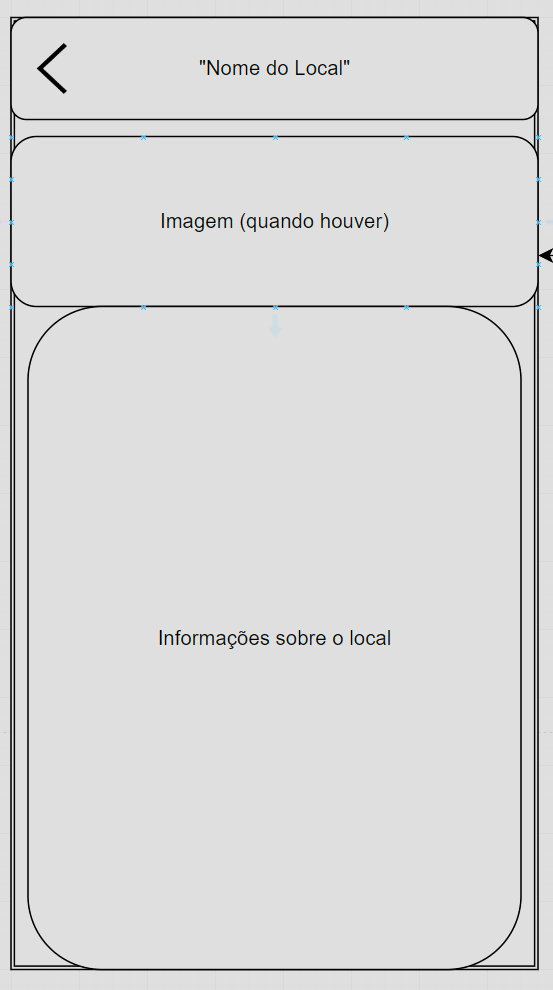
\includegraphics[width=0.2\linewidth]{images/wire-tela-local.png}\\
  \end{center}
  \caption[Wireframe Tela Local]{Wireframe Tela Local}
  \label{fig:wireframe-tela-local}
  \legend{Fonte: Próprio Autor}
\end{figure}
Na tela local será possível visualizar na tela a imagem de um determinado local buscado(quando houve) sempre na parte superior da tela acima das informação em formato de texto. 

Haverá uma app bar onde o título deverá apresentar o nome do local. Essa app bar estará posicionada sempre no início da tela. Ela conterá um ícone de seta virada para esquerdade que remete a ação de voltar a tela nos aplicativos.
\begin{comment}
\begin{alineas}
  \item Tipo de interface e interação
  
Na tela lugar será utilizada o tipo de tela de interface gráfica onde o usuário irá visualizar informações sobre o local que ele clicou na tela home. A forma de interação será através de toque no botão de voltar para retroceder a tela home. 
  \item Metáforas
  
Ícone de seta para esquerda indicando a ação de voltar na tela. O ícone estará presente no toolbar da tela no canto superior esquerdo como é de costume em aplicações mobile.
  \item Aprendizibilidade
  
Previsibilidade – Ao clicar no ícone da seta para esquerda espera-se que retroceda uma tela.

Capacidade de sintetização – Não se aplica.

Familiaridade – Não se aplica.

Consistência – O ícone de voltar aparecerá sempre no mesmo local, ou seja, canto superior esquerdo.

Generalização – Não se aplica.

  \item Flexibilidade
  
Iniciativa de diálogo – Não se aplica.

Multitarefa – Não se aplica.

Substitutividade – Não se aplica.

Personalização – Não se aplica.


  \item Robustez
  
 Observabilidade – Os dados apresentados na tela serão do local escolhido na busca na tela anterior.
 
Recuperabilidade – O sistema irá emitir um alert em formato de Toast indicando quando houver falha no envio de um pedido de socorro e pedirá para que o usuário refaça a solicitação.

Capacidade de resposta – Não se aplica.

Conformidade de realização de atividades – Não se aplica. 
\end{alineas}
\end{comment}
\subsection{Tela 3 - Perfil}
\begin{figure}[h]
  \begin{center}
  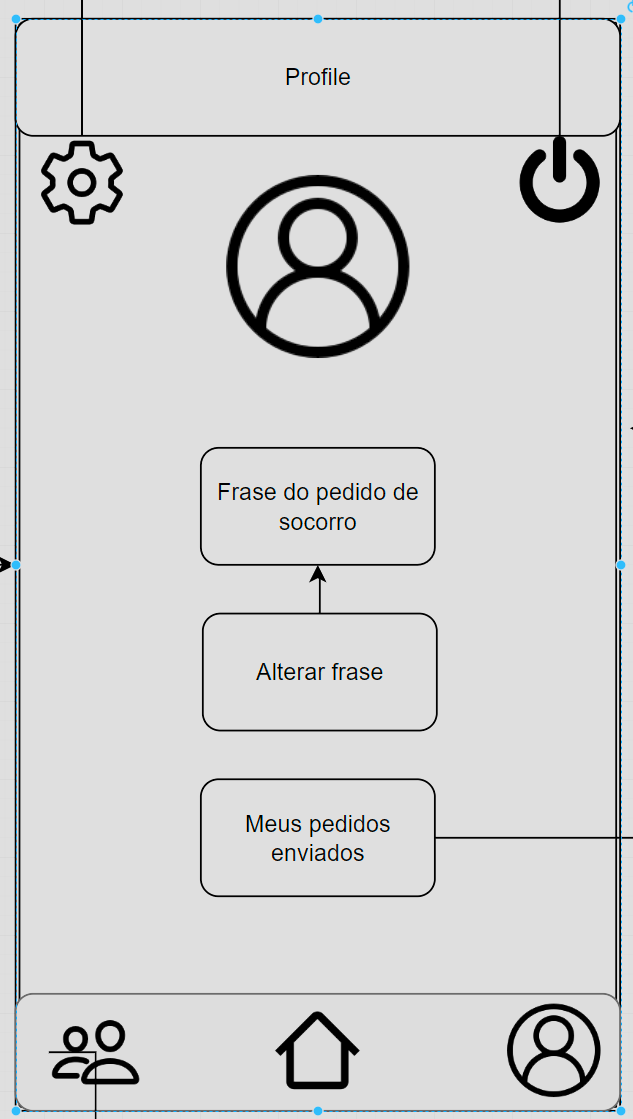
\includegraphics[width=0.2\linewidth]{images/wire-tela-perfil.png}\\
  \end{center}
  \caption[Wireframe Tela Perfil]{Wireframe Tela Perfil}
  \label{fig:wireframe-tela-perfil}
  \legend{Fonte: Próprio Autor}
\end{figure}
\pagebreak
O título da tela será sempre apresentado no início da tela.  Na tela de perfil será apresentado dois icone um de engrenagem que remete ao acesso a área de configurações em qualquer aplicativo e também o ícone de power off que remete a ação de logar/deslogar de qualquer aplicativo. 

Abaixo do título da tela será exibida a imagem de perfil do usuário(quando houver) ou um ícone padrão de perfil(quando não houver).

Será exibido a frase do pedido se soccoro(frase padrão até ser editada pelo usuário) a ser enviada e apresentado um botão para acionamento da edição desta frase para um texto pessoal definido pelo usuário. 

Abaixo da frase será exibido os ultimos pedidos de socorro enviados ou um frase de alert no caso de nenhum pedido tenha sido enviado. Nesta mesma área será possível acionar através de toque um botão que levará o usuário para a ela onde poderá acessar todos os pedidos que ele já enviou visto que nesta tela serão apresenados apenas os últimos pedidos.
\begin{comment}
\begin{alineas}
  \item Tipo de interface e interação
  
Na tela de perfil será utilizada o tipo de tela de interface gráfica com multi toque. A forma de interação será através de multi toque, onde ao clicar nas opções disponíveis na tela será possível realizar a ação correspondente. 
  \item Metáforas
  
A BottomBar contém ícones os quais remetem as funcionalidades do aplicativo. O ícone com dois bonecos remete a uma lista de contatos. O ícone da casa remete a tela principal de qualquer aplicativo. Já o ícone circular com boneco dentro remete ao perfil em qualquer aplicação. A própria BottomBar já remete a ideia de que é possível navegar entre essas três telas sem que tenha que sair deste menu em si. Há também dois botões de ícones que indicam configurações(engrenagem) e logoff(power).
  \item Aprendizibilidade
  
Previsibilidade – Ao alterar a mensagem do pedido de socorro o usuário recebe um alert em forma de Toast indicando que a alteração foi concluída com sucesso. 

Capacidade de sintetização – Após alterar a mensagem de pedido de socorro a nova mensagem é automaticamente exibida na área da tela onde a mensagem é mostrada.

Familiaridade – Não se aplica.

Consistência – Após a alteração da mensagem de pedido de socorro, os novos pedidos enviados devem ser emitidos com a nova mensagem. Não há alterações para os pedidos já enviados anteriormente.

Generalização – Não se aplica.

  \item Flexibilidade
  
Iniciativa de diálogo – Não se aplica.

Multitarefa – Não se aplica.

Migração de atividades – Caso o usuário altere a mensagem e não clique em salvar, ao sair do foco do campo de inserir a mensagem, o conteúdo atual é salvo como nova mensagem.

Substitutividade – Não se aplica.

  \item Robustez
  
Observabilidade – O usuário irá ver automaticamente a nova mensagem de pedido de socorro assim que ele salvar a sua edição.

Recuperabilidade – Não se aplica.

Capacidade de resposta – Não se aplica.

Conformidade de realização de atividades – Não se aplica

\end{alineas}
\end{comment}
\subsection{Tela 4 - Configurações}
\begin{figure}[h]
  \begin{center}
  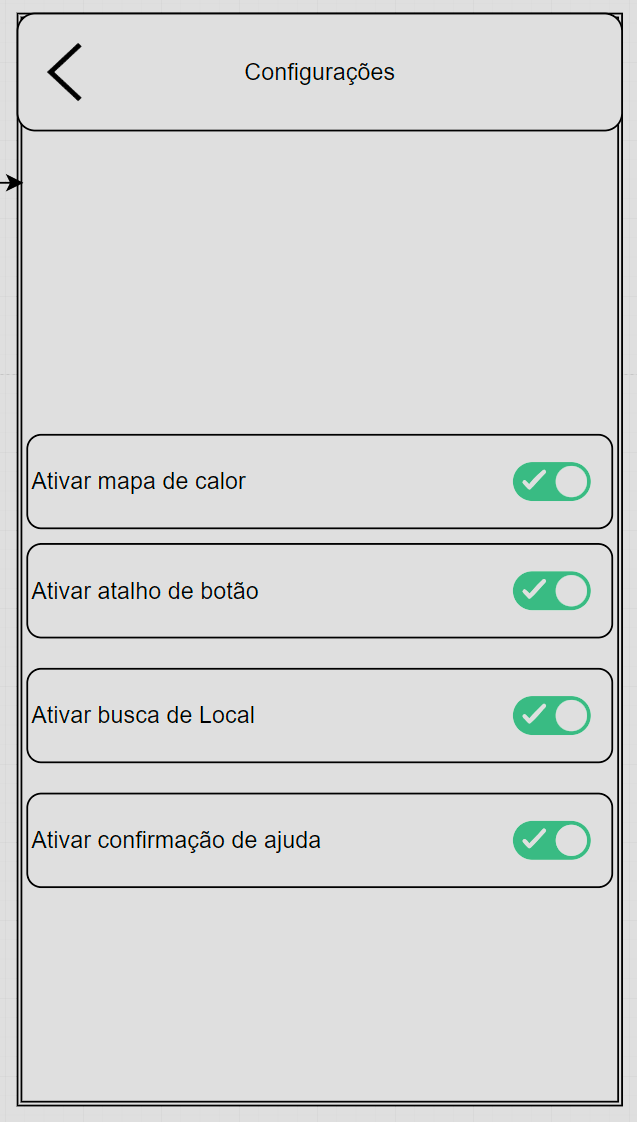
\includegraphics[width=0.2\linewidth]{images/wire-tela-configuracoes.png}\\
  \end{center}
  \caption[Wireframe Tela Configurações]{Wireframe Tela Configurações}
  \label{fig:wireframe-tela-configuracoes}
  \legend{Fonte: Próprio Autor}
\end{figure}
\pagebreak
Na tela de configurações serão apresentadas as customizações que serão possíveis realizar no aplicativo. Através de switch toggles, que remete a liga e desliga, o usuário será capaz de ativar ou desativar as customizações possíveis da aplicação. O usuário poderá realizar o acionamento do switch através de clique ou através de gesto de arrastar a chave para a nova posição.
\begin{comment}
\begin{alineas}
  \item Tipo de interface e interação
  
O tipo de interface será de central de controle, onde o usuário será capaz de ativar ou desativar alguns recursos e configurações do aplicativo. 
A interação será através de gesto de deslize para ativar ou desativar as chaves para cada configuração presente na tela.

  \item Metáforas
  
Os toggles dão ideia de um interruptor para desligar ou ligar a configuração respectiva.
  \item Aprendizibilidade
  
Previsibilidade – Ao acionar o toggle o sistema emitirá alertas de que a respectiva funcionalidade foi liga ou desligada.

Capacidade de sintetização – Não se aplica.

Familiaridade – Os toggle remetem ao interruptor da vida real. 

Consistência – Não se aplica.

Generalização – Não se aplica.

  \item Flexibilidade
  
Iniciativa de diálogo – Não se aplica.

Multitarefa – Não se aplica.

Migração de atividades – Não se aplica.

Substitutividade – Não se aplica.

Personalização – Não se aplica.

  \item Robustez
  
Observabilidade – Ao acionar o toggle de alguma das funcionalidades o usuário será capaz de ver imediatamente o novo estado desta funcionalidade, se está ativada ou não.

Recuperabilidade – Não se aplica.

Capacidade de resposta – Um alert em formato Toast será exibido cada vez em que o estado de uma das funcionalidades for alterado entre liga e desliga.

Conformidade de realização de atividades – Não se aplica
\end{alineas}
\end{comment}
\subsection{Tela 5 - Tela Cadastro contato seguro}
\begin{figure}[h]
  \begin{center}
  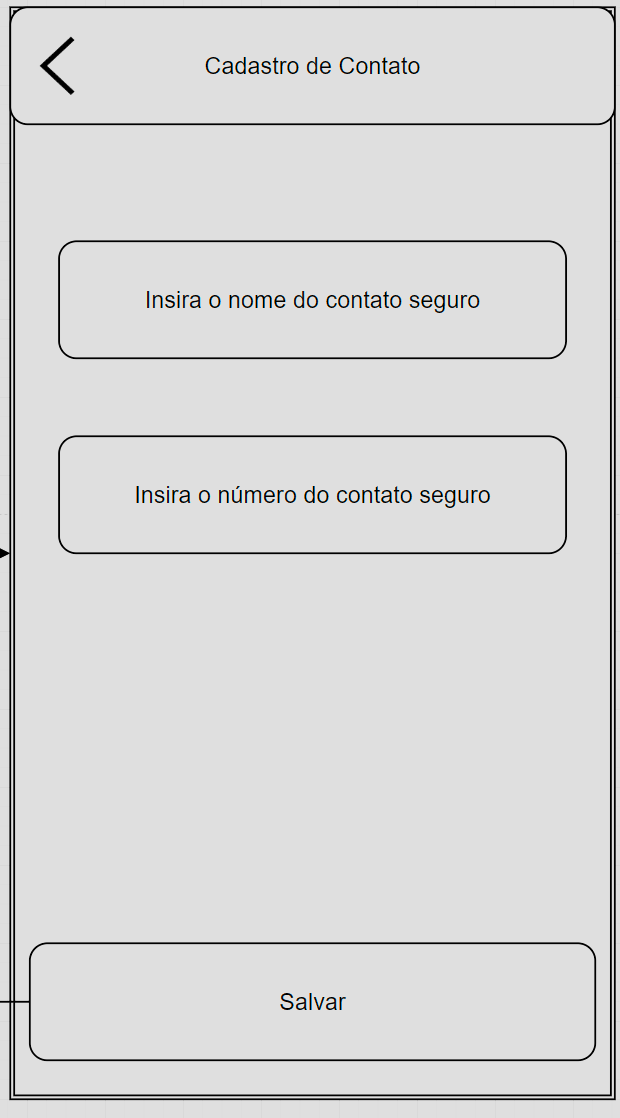
\includegraphics[width=0.2\linewidth]{images/wire-tela-cadsatro-contato-seguro.png}\\
  \end{center}
  \caption[Wireframe Tela Cadastro contato seguro]{Wireframe Tela Cadastro contato seguro}
  \label{fig:wireframe-tela-cadastro-contato-seguro}
  \legend{Fonte: Próprio Autor}
\end{figure}
\pagebreak
Será apresentado um formulário onde o usuário será capaz de inserir os dados do seu contato seguro. Para interação com o formulário o usuário deverá clicar em cada um dos campos para inserção dos dados. Alertas de erros nos campos serão exibidos quando o usuário tentar enviar o formulário com dados inválidos(formulário com dados vazios, dígitos no campo de nome). 

Através do botão salvar os dados serão enviados para cadastramento na base de dados. Será exibidada um tela de carregamento enquanto os dados estirevem em transferência para base de dados, mantendo assim o usuário informado sobre a sua ação de salvamento. O mesmo formulário também será utilizado para edição do contato seguro. Neste cenário as dados do cadastro já viram preenchidos e o usuário poderá alterar tais dados.

Através do ícone da seta para a esquerda, assim como nas outras telas em que aparece, o usuário será capaz de retornar a tela anterior. 
\begin{comment}
\begin{alineas}
  \item Tipo de interface e interação
  
A interface será do tipo formulário onde o usuário deverá preencher os dados para cadastro do contato seguro. O tipo de interação será através de preenchimento de campos.
  \item Metáforas
  
Um botão com ícone de seta para esquerda será exibido na app bar indicando a ação de voltar para tela anterior.
  \item Aprendizibilidade
  
Previsibilidade – Um alert em forma de Toast será exibido ao salvar com sucesso um contato.

Capacidade de sintetização – Ao salvar o novo contato com sucesso a tela de listagem de contatos deverá exibir a listagem já com o novo contato inserido na tela. 

Familiaridade – O contato seguro remete a um contato de telefone na agenda do usuário.

Consistência – Não se aplica.

Generalização – Não se aplica
  \item Flexibilidade
  
Iniciativa de diálogo – Não se aplica.

Multitarefa – Não se aplica.

Migração de atividades – Não se aplica.

Substitutividade – Não se aplica.

Personalização – Não se aplica.
  \item Robustez
  
Observabilidade – Não se aplica.

Recuperabilidade – Caso não consiga realizar o cadastro o sistema emitirá um alert em formato de Toast pedindo para o que o usuário refaça a operação.
 
Capacidade de resposta – Será emitido um alerta em formato de Toast informando ao usuário o cadastro no novo contato seguro.

Conformidade de realização de atividades – Ao tentar salvar um novo contato seguro com dados inválidos, por exemplo nome e número de telefone em branco, o usuário receberá uma notificação no campo referido para que faça a correção dele. O mesmo acontecerá caso ele tente adicionar um contato que já esteja salvo na sua lista de contatos seguros. 

\end{alineas}
\end{comment}
\subsection{Tela 6 - Tela Listagem de contatos}
\begin{figure}[h]
  \begin{center}
  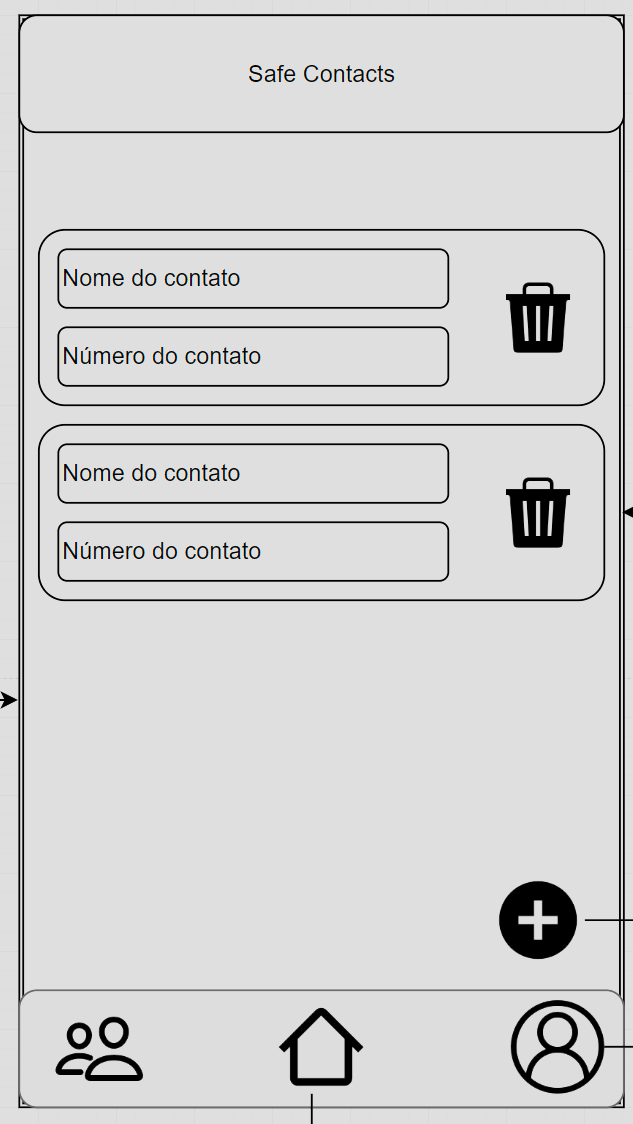
\includegraphics[width=0.2\linewidth]{images/wire-tela-listagem-contatos.png}\\
  \end{center}
  \caption[Wireframe Tela Listagem de contatos]{Wireframe Tela Listagem de contatos}
  \label{fig:wireframe-tela-listagem-contatos}
  \legend{Fonte: Próprio Autor}
\end{figure}
\pagebreak
Na tela de listagem de contatos será exibidos alista de contatos seguros queo usuário já cadastrou no aplicatiov. Caso não haja nenhum contato cadastrado será exibida uma mensagem informativa de que ainda não foram cadsatrados contatos. 

Há um float action buttoncom ícone de + que remete a ação de adicionar algo em qualquer aplicativo. A interação é através do clique no botão que levará para a tela de cadastro do novo contato.

Os contatos serão exibidos em forma de lsitagem na tela onde cada contato teerá seu próprio card exibido. Cada card exibirá o nome e o telefone do contato seguro cadastrado, desta forma o usuário conseguirá identificar sem equívoco cada um dos seus contatos. Haverá um menu de contexto o qual a ser clicado o usuário conseguirá acessar as funções de editar e deletar os conttos já cadastrados. Uma vez que o wireframa foi utilizado nesta análise, o menu de ocntexto será possível ser visualizado na imagem do prótotipo final. 

A tela seguirá o mesmo padrão das telas principais, mantendo a bottom bar no final da tela com os três ícones das funcionalidades principais indicando a navegação. 
\begin{comment}
	\begin{alineas}
		\item Tipo de interface e interação
		
		O tipo de interface utilização será de interface gráfica com listagem. A interação será feita através de gesto de rolagem na tela e com clique para ações. 
		\item Metáforas
		
		A BottomBar contém ícones os quais remetem as funcionalidades do aplicativo. O ícone com dois bonecos remete a uma lista de contatos. O ícone da casa remete a tela principal de qualquer aplicativo. Já o ícone circular com boneco dentro remete ao perfil em qualquer aplicação. 
		
		A própria BottomBar já remete a ideia de que é possível navegar entre essas três telas sem que tenha que sair deste menu em si.
		O ícone de lixeira será utilizado em cada card de contato indicando que ao clicar ali será executada a ação de deleção do contato seguro correspondente.
		
		\item Aprendizibilidade
		
		Previsibilidade – Ao clicar na lixeira de um determinado contato seguro o usuário receberá um alert em forma de Toast indicando que o contato seguro foi deletado.
		
		Capacidade de sintetização – Ao excluir um contato seguro com sucesso a tela de listagem de contatos é atualizada para retirar o contato seguro que foi removido.
		
		Familiaridade – Não se aplica.
		
		Consistência – Não se aplica. 
		
		Generalização – Não se aplica.
		
		\item Flexibilidade
		
		Iniciativa de diálogo – Não se aplica.
		
		Multitarefa – Não se aplica.
		
		Migração de atividade – Não se aplica.
		
		Substitutividade – Não se aplica.
		
		Personalização – Não se aplica.
		
		\item Robustez
		
		Observabilidade – Ao excluir um contato com sucesso o estado da tela de listagem é atualizado com a nova lista sem o contato que foi deletado.
		
		Recuperabilidade – O contato somente é deixado de ser exibido caso tenha ocorrido com sucesso a deleção. Em caso de insucesso é exibido um alerta em formato de Toast para o usuário indicando para que ele refaça a operação.
		
		Capacidade de resposta – Será exibido para o usuário um alerta em formato Toast indicando a deleção do contato seguro.
		
		Conformidade de realização de atividades – Não se aplica
	\end{alineas}
\end{comment}

\subsection{Tela 7 - Tela Pedidos de ajuda enviados}
\begin{figure}[h]
  \begin{center}
  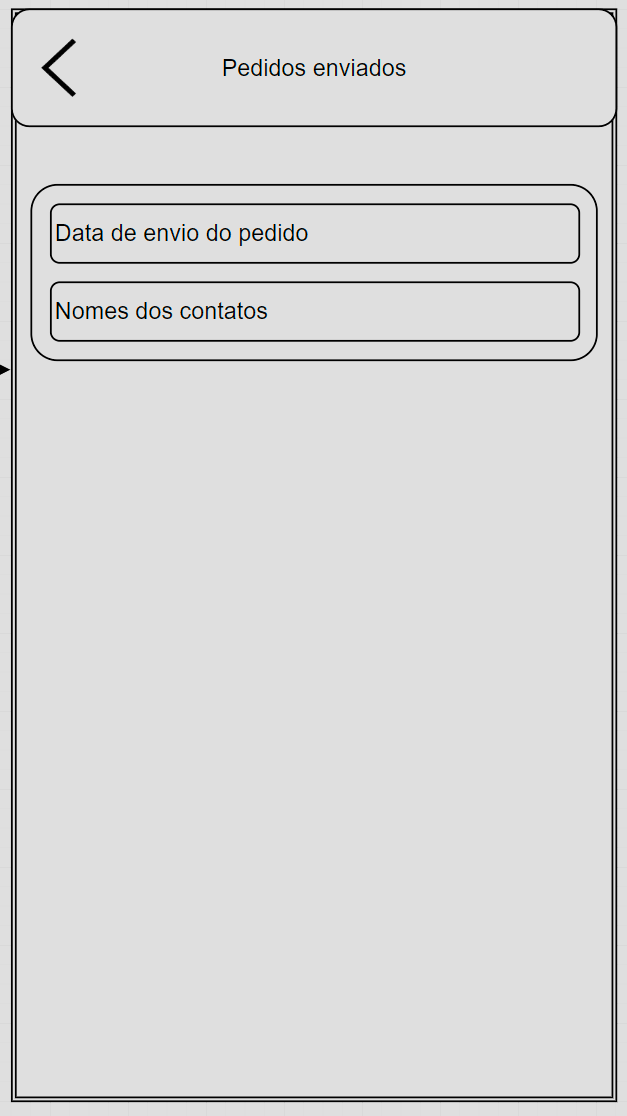
\includegraphics[width=0.2\linewidth]{images/wire-tela-pedidos-enviados.png}\\
  \end{center}
  \caption[Wireframe Tela Pedidos de ajuda enviados]{Wireframe Tela Pedidos de ajuda enviados}
  \label{fig:wireframe-tela-pedidos-ajuda}
  \legend{Fonte: Próprio Autor}
\end{figure}
\clearpage
\begin{comment}
\begin{alineas}
  \item Tipo de interface e interação
  
Será utilizada nessa tela o tipo de interface de listagem. A interação será através de scroll na tela. 
  \item Metáforas
  
Botão com ícone de seta para esquerda será exibido no canto superior esquerdo da AppBar indicando que irá retornar para tela anterior.
  \item Aprendizibilidade
  
Previsibilidade – Não se aplica.

Capacidade de sintetização – Não se aplica

Familiaridade – Não se aplica.

Consistência – Não se aplica.

Generalização – Não se aplica.
  \item Flexibilidade
  
Iniciativa de diálogo – Não se aplica.

Multitarefa – Não se aplica.

Migração de atividade – Não se aplica.

Substitutividade – Não se aplica.

Personalização – Não se aplica.

  \item Robustez
  
Observabilidade – Não se aplica.

Recuperabilidade – Ao obter erro na busca dos pedidos de socorro enviado do usuário, será emitido um alerta em forma de Toast indicando o erro e pedindo para que ele saia e entre novamente na tela de listagem. 

Capacidade de resposta – Indicar ao usuário quando não houver dados na listagem para serem exibidos.

Conformidade de realização de atividades – Não se aplica.

\end{alineas}
\end{comment}
Nesta tela serão exibidos os pedidos de socorro enviados em forma de listagem. Cada pedido será identificado em um card. Neste card conterá a data do pedido enviado e a localização de onde ele foi enviado. Será possível clicar no link das coordenadas de localização e ser direcionado para o aplicativo de mapas do usuário. O link será exibido com um sublinhado indicando que é um elemento clicável como acontece em qualquer aplicativo.
\begin{comment}
\section{Avaliação realizadas}
\subsection{Respostas das avaliações}
Os documentos contendo as avaliações dos herísticas e rasteiras dos avaliadores podem ser encontradas no Anexo A deste documento.

Os documentos contendo as avaliações de acessibilidae dos avaliadores podem ser encontrados no Anexo B deste documento.

\end{comment}

\section{Avaliação com usuário}
A avaliação com usuário constitui-se como um paradigma metodológico fundamental no campo da Interação Humano-Computador (IHC), caracterizado pela participação direta de usuários reais no processo de análise e validação de sistemas interativos \cite{dix2003human}. Esta abordagem fundamenta-se no princípio de que a qualidade de um sistema deve ser mensurada a partir da perspectiva de quem efetivamente o utiliza, considerando suas necessidades, expectativas, limitações cognitivas e contextos de uso específicos \cite{preece2015interaction}.

Diferentemente dos métodos de inspeção realizados por especialistas, a avaliação com usuário oferece insights diretos sobre a experiência real de interação, revelando aspectos que podem não ser identificados através de análises teóricas ou heurísticas \cite{nielsen1994usability}. Esta metodologia permite a observação de comportamentos autênticos, identificação de estratégias de uso não previstas pelos designers, e compreensão das dificuldades reais enfrentadas pelos usuários em contextos naturais de utilização.

\subsection{Avaliação do usuário SheSafe}
As avaliações com usuário da aplicação SheSafe foram conduzidas entre os dias 24 e 28 de setembro de 2025, envolvendo participantes que executaram três tarefas específicas relacionadas às funcionalidades principais do sistema. Os testes foram realizados com a versão debug da aplicação Android, disponibilizada através de um link de download compartilhado.

Em relação ao cumprimento dos objetivos das tarefas, os resultados demonstraram 100\% de taxa de sucesso, com todas as participantes conseguindo completar as três atividades propostas: enviar um pedido de socorro pela primeira vez, cadastrar um novo contato seguro e alterar a mensagem padrão do pedido de ajuda. Não foram registrados erros durante a execução de nenhuma das tarefas, indicando que a interface apresenta boa intuitividade e que os fluxos de interação estão adequadamente projetados para facilitar a conclusão das ações pelos usuários.

A análise dos tempos de execução revelou performance satisfatória em todas as tarefas avaliadas. Para o envio do primeiro pedido de socorro, os tempos variaram entre 21 e 31 segundos, com média de 25,3 segundos. O cadastro de contatos seguros apresentou tempos mais consistentes, variando entre 13 e 17 segundos (média de 14,3 segundos). A alteração da mensagem padrão foi a tarefa executada mais rapidamente, com tempos entre 11 e 14 segundos (média de 12,3 segundos). Esta progressão temporal sugere que as funcionalidades mais críticas mantêm tempos de resposta adequados para situações de emergência, enquanto as funcionalidades de configuração são executadas de forma ainda mais eficiente.

No que se refere às impressões qualitativas, as avaliadoras expressaram percepções predominantemente positivas sobre diferentes aspectos da aplicação. A navegação foi consistentemente avaliada como adequada por todas as participantes, assim como o design visual e a usabilidade geral do sistema.
\begin{comment}
	Mônica Abreu destacou especificamente que "a interface é muito fácil e simples de aprender a utilizar", enquanto Wannielly Barbosa elogiou a "navegação fluida e sem problema para mudar de tela", caracterizando ainda a iniciativa como "ótima para mulheres".
\end{comment}

Contudo, emergiu um padrão consistente de feedback relacionado à ausência de confirmações explícitas do sistema após a execução de determinadas ações. Algumas das avaliadoras relataram especificamente a "falta de um retorno ao cadastrar o contato", enquanto uma outra observou que "ao alterar mensagem, só vi que alterou quando mudou na tela". Este feedback indica uma oportunidade de melhoria significativa no design de interação, particularmente na implementação de feedback imediato e explícito para ações críticas do usuário.

A convergência deste feedback específico sobre a ausência de confirmações do sistema sugere que esta deficiência pode impactar negativamente a confiança do usuário na aplicação, especialmente em um contexto de uso onde a certeza sobre a execução correta das ações é fundamental para a eficácia do sistema de segurança. A implementação de mensagens de confirmação, notificações toast, ou outros elementos de feedback visual imediato deveria ser considerada como prioridade para futuras iterações do desenvolvimento, visando aumentar a transparência do sistema e a confiança do usuário nas operações realizadas.

\section{Correções e melhorias}
O protótipo se mostrou muito agradável aos participantes das avaliações. Alguns foram elencados e foram trabalhados para que acontecessem as devidas alterações. Alguns pontos foram bastante mencionados na avaliação heurísticas e rasteira. Sendo eles: 
\begin{itemize}
\item Alteração de contato – Foi adicionado um menu de contexto que apresentará a opção de edição do contato já salvo para que não seja preciso excluir um contato primeiro para depois adicionar seu novo número.
\item Exclusão de contato – Foi adicionada uma confirmação para prevenir de uma exclusão de contato acidental.
\item Configurações – Foi alterado o título da tela de configurações para corresponder com a tela.
\item Ícone de logout – Foi alterado o ícone para ficar mais intuitivo. 
\item Alteração de mensagem padrão – Foi adicionado um feedback após realizar a alteração da mensagem para que fique mais claro de que a ação ocorreu com sucesso.
%\item Campo de busca – Será adicionado um hint ao campo de busca informando o que o usuário deve preencher.
\item Botões de voltar – Foi descrescido o tamnaho dos ícones de voltar nas telas que possuem.
\end{itemize}
 
Uma nova heurística que foi introduzida na aplicação SheSafe foi o login com redes sociais. Hoje em dia é sim muito comum já termos essa opção nos aplicativos, porém ainda existem aqueles que não possuem essa funcionalidade. O login da aplicação SheSafe é feito através da conta Google, e com o tempo a ideia é implementar o login com mais redes sociais.

No quesitos das avaliações de acessibilidade foi possível perceber que o protótipo atendeu as epectativas de quem o avaliou. Apesar de poucos apontamentos alguns deles se tornaram bastante perceptíveis visto que mais de um avaliador comentou sobre o mesmo problema. Desta forma as seguintes alterações foram realizadas.

\begin{itemize}
\item Alteração do nome da Tela 7 para condizer e identificar unicamente a tela de configurações
%\item Criação de tooltip para cada menu de ação na tela 6 para assim melhor informar o que cada menu faz
%\item Atentar ao uso do mapa na codificação para garantia de permissões necessárias.
%\item Aplicar hint ao campo de busca para melhor definição do que se espera como entrada
\item Adicionado tolltip ao botão de adicionar contato seguro para melhor acessibilidade
\item Melhorara da formatação dos rótulos dos campos do formulário de cadastro de contato
\item Aplicação de visual de link na listagem de pedidos enviados na tela 8
\item Reavaliado o contraste dos botões dos dialogs
\end{itemize}

